\documentclass[10pt]{article}
\usepackage[margin=1.25in]{geometry}
\usepackage{amsmath,amssymb,amsthm,mathtools}
\usepackage{microtype}
\usepackage{graphicx}
\usepackage[hidelinks]{hyperref}
\usepackage{enumitem}
\setlist{leftmargin=1.15em,itemsep=0.15em,topsep=0.25em}
\setlength{\parindent}{0pt}
\setlength{\parskip}{0.48em}

\newtheorem{theorem}{Theorem}
\newtheorem{proposition}{Proposition}
\newtheorem{corollary}{Corollary}
\newtheorem{definition}{Definition}

\begin{document}

\begin{center}
{\LARGE \bfseries The Entropy of Finite Response\par}
\vspace{0.35em}
{\large Causal kernels, closure, and spread\par}
\vspace{1.2em}
{\large J. Landers\par}
\vspace{0.5em}
{Draft note\par}
\end{center}

\vspace{0.8em}

\begin{abstract}
Idealized models often describe a response as instantaneous. This note separates the source from the physical mediator: the observed response is the source convolved with a passive causal kernel. Such kernels have two elementary operations, convex mixing for parallel channels and convolution for sequential stages. The resulting moment laws show that hidden passive stages cannot sharpen an already mediated response; sharpness lives only on a singular boundary of the kernel space. Replacing variance by entropy power makes the statement strict: by the entropy power inequality and the support constraint imposed by causality, every nontrivial sequential stage increases entropy power by more than simple additivity would predict. The causal interior is therefore pinned between two unreachable walls---the delta locus $N=0$ and the Gaussian locus $N=\sigma^2$---with real finite-response dynamics living between them.
\end{abstract}

\section{From instantaneous onset to mediated response}

Let an idealized force or source field be written as
\[
F_{\mathrm{ideal}}(x,t),
\]
where $x\in\mathbb R^d$ is position and $t$ is time. A physically observed response may be modeled as
\begin{equation}\label{eq:general_kernel}
F_{\mathrm{actual}}(x,t)
=
\int_{\mathbb R^d}\int_{-\infty}^{t}
G(x-x',t-s)F_{\mathrm{ideal}}(x',s)\,ds\,dx'.
\end{equation}
Here $G$ is the mediation kernel. The source $F_{\mathrm{ideal}}$ is what is being mediated; the kernel $G$ describes how mediation occurs. In compact notation,
\[
F_{\mathrm{actual}}=G*F_{\mathrm{ideal}}.
\]
This source--kernel separation is the organizing move of the note; the convolution algebra is standard, but here it is used to isolate what finite passive response does to sharpness.

This formalism captures the distinction between an idealized onset and a finite physical response. If $m\ddot x=F$ and one writes an ideal step force
\[
F(t)=F_0H(t-t_0),
\]
then
\[
a(t)=\frac{F_0}{m}H(t-t_0),\qquad
j(t)=\dot a(t)=\frac{F_0}{m}\delta(t-t_0).
\]
Thus an instantaneous onset of acceleration corresponds, in the distributional sense, to an impulse in jerk. A causal temporal kernel $K$ replaces this singularity by finite response:
\begin{equation}\label{eq:temporal}
F_{\mathrm{actual}}(t)=\int_{-\infty}^{t}K(t-s)F_{\mathrm{ideal}}(s)\,ds,
\qquad K(t)=0\;\text{for }t<0.
\end{equation}
For the step source,
\[
F_{\mathrm{actual}}(t)=F_0\int_0^{t-t_0}K(u)\,du,
\qquad
j(t)=\frac{F_0}{m}K(t-t_0).
\]
So the singular idealization
\[
\delta(t-t_0)
\]
is replaced by the finite kernel
\[
K(t-t_0).
\]

\section{Two canonical geometries}

The kernel formalism separates the source from the transport geometry. Two limiting cases are especially useful: sharp transport on an arrival surface and diffusive transport through a broadening profile.

\textbf{Ballistic mediation.} In three spatial dimensions, a sharp finite-speed wavefront is represented by
\begin{equation}\label{eq:ballistic}
G_{\mathrm{ballistic}}(x-x',t-s)
=
\frac{1}{4\pi r}
\delta\!\left((t-s)-\frac{r}{c}\right)H(t-s),
\qquad r=\|x-x'\|.
\end{equation}
This kernel has response concentrated at the arrival time $t-s=r/c$. It is not instantaneous; it is a delayed sharp arrival.

\textbf{Diffusive mediation.} In $d$ dimensions, a diffusion-like response is represented by
\begin{equation}\label{eq:diffusive}
G_{\mathrm{diffusive}}(x-x',t-s)
=
\frac{H(t-s)}{(4\pi D(t-s))^{d/2}}
\exp\!\left(-\frac{\|x-x'\|^2}{4D(t-s)}\right),
\end{equation}
where $D>0$ is the diffusion coefficient. This kernel spreads influence over a length scale
\[
\ell(t-s)\sim \sqrt{D(t-s)}.
\]
The ballistic kernel lives on a sharp arrival surface; the diffusive kernel fills space-time with a broadening cloud. Both are choices of $G$ in Eq.~\eqref{eq:general_kernel}, and the diffusive case later connects this finite-response picture to the entropy--Fisher-information identities used in information theory \cite{dembo1991}.

\section{Kernel space: mixtures and compositions}

There are two elementary ways to build a complicated mediation law from simpler ones.

First, distinct channels may act in parallel:
\begin{equation}\label{eq:mixture}
G_\lambda=(1-\lambda)G_1+\lambda G_2,
\qquad 0\le \lambda\le 1.
\end{equation}
For example, a direct ballistic channel may coexist with a scattered diffusive tail:
\[
G_\lambda=(1-\lambda)G_{\mathrm{ballistic}}+
\lambda G_{\mathrm{diffusive}}.
\]
Second, mediation stages may occur sequentially. If the source first passes through $G_1$ and then through $G_2$, the total kernel is
\begin{equation}\label{eq:composition}
G_{\mathrm{total}}=G_2*G_1.
\end{equation}
Thus addition represents parallel physical channels, while convolution represents cascaded physical stages.

This suggests that physically admissible kernels form not a single family but a structured space: a constrained set closed under convex mixing and, under suitable assumptions, closed under composition. If one requires composition at all subdivision scales, this is the language of convolution semigroups familiar from Levy-process theory \cite{applebaum2009}; here only the finite two-stage version is needed. The following proposition makes the simplest temporal version precise.

\section{A small closure and spread result}

\begin{definition}[Passive causal temporal kernel]
A kernel $K$ is passive causal if
\[
K(t)=0\text{ for }t<0,\qquad K(t)\ge 0,
\qquad \int_0^\infty K(t)\,dt=1,
\]
and if its first two moments are finite. Define
\[
\mu(K)=\int_0^\infty tK(t)\,dt,
\qquad
\sigma^2(K)=\int_0^\infty (t-\mu(K))^2K(t)\,dt.
\]
\end{definition}

\begin{proposition}[Causal mediation spread]\label{thm:spread}
Let $K_1$ and $K_2$ be passive causal temporal kernels.

\emph{Parallel channels.} For
\[
K_\lambda=(1-\lambda)K_1+\lambda K_2,
\qquad 0\le\lambda\le1,
\]
$K_\lambda$ is passive causal, and
\begin{equation}\label{eq:mean_mix}
\mu(K_\lambda)=(1-\lambda)\mu(K_1)+\lambda\mu(K_2),
\end{equation}
\begin{equation}\label{eq:var_mix}
\sigma^2(K_\lambda)
=(1-\lambda)\sigma^2(K_1)+\lambda\sigma^2(K_2)
+\lambda(1-\lambda)\bigl(\mu(K_2)-\mu(K_1)\bigr)^2.
\end{equation}

\emph{Sequential stages.} For
\[
K_{\mathrm{total}}=K_2*K_1,
\]
$K_{\mathrm{total}}$ is passive causal, and
\begin{equation}\label{eq:mean_conv}
\mu(K_2*K_1)=\mu(K_1)+\mu(K_2),
\end{equation}
\begin{equation}\label{eq:var_conv}
\sigma^2(K_2*K_1)=\sigma^2(K_1)+\sigma^2(K_2).
\end{equation}
\end{proposition}

\begin{proof}
Since nonnegative causal normalized functions are probability densities on $[0,\infty)$, interpret $K_i$ as the delay distribution of a nonnegative random variable $T_i$. A convex mixture first chooses channel $1$ with probability $1-\lambda$ and channel $2$ with probability $\lambda$. Equations \eqref{eq:mean_mix} and \eqref{eq:var_mix} are the standard laws of total expectation and total variance.

For sequential stages, the total delay is
\[
T_{\mathrm{total}}=T_1+T_2,
\]
with independent stages. The density of $T_1+T_2$ is $K_2*K_1$. Since $T_1,T_2\ge0$, the convolution remains causal; normalization follows by Fubini's theorem. The expectation and variance of the sum give \eqref{eq:mean_conv} and \eqref{eq:var_conv}, as illustrated by the exponential cascade in Fig.~\ref{fig:convolution-cascade}.
\end{proof}

\begin{figure}[t]
\centering
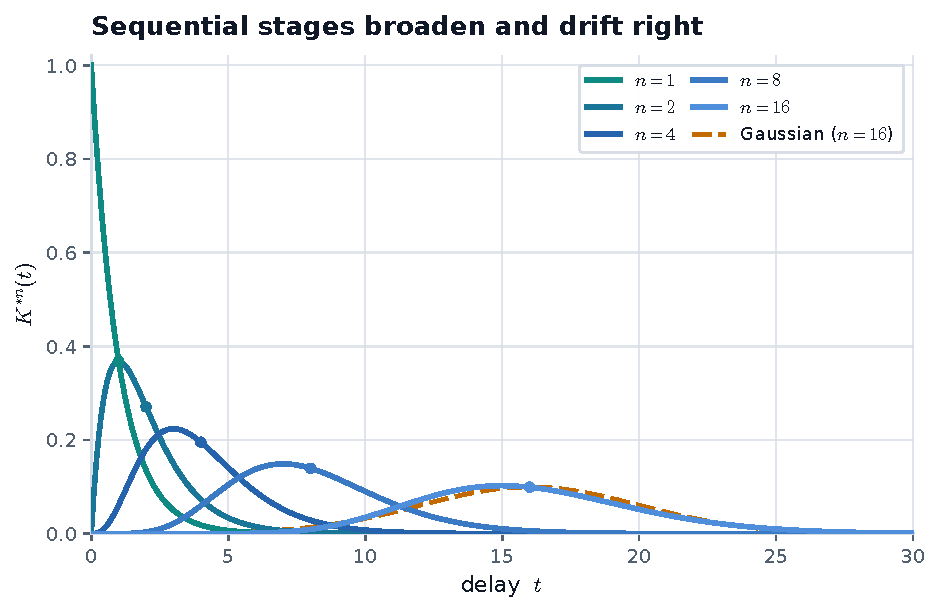
\includegraphics[width=\linewidth]{fig2_convolution_cascade.pdf}
\caption{Sequential stages broaden and drift. Self-convolution of an exponential, $\Gamma(1,\theta)^{*n}=\Gamma(n,\theta)$, realizes the additive laws of Proposition~\ref{thm:spread} ($\mu=n$, $\sigma^2=n$ at $\theta=1$). The shape approaches a Gaussian in the usual convolution limit \cite{barron1986} but stays causal; the matched Gaussian for $n=16$ (dashed) lies strictly outside on $t<0$.}
\label{fig:convolution-cascade}
\end{figure}

The proposition formalizes a simple physical intuition: hidden passive stages accumulate delay and spread. A delta delay, $K(t)=\delta(t-t_0)$, has zero variance and lies on the sharp boundary of the space. Any nontrivial stage with positive variance makes the response less instantaneous. Parallel mixtures may also broaden a response even if each channel is individually sharp, as shown in Fig.~\ref{fig:parallel-mixture}, because different arrival times produce the additional term in Eq.~\eqref{eq:var_mix}.

\begin{figure}[t]
\centering
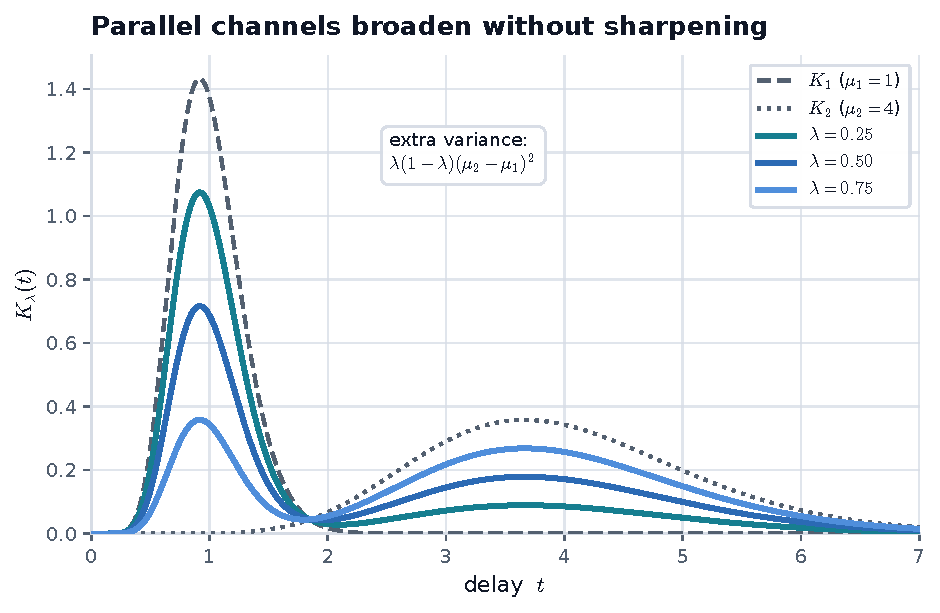
\includegraphics[width=\linewidth]{fig3_parallel_mixture.pdf}
\caption{Parallel channels broaden without sharpening. Convex mixtures $K_\lambda=(1-\lambda)K_1+\lambda K_2$ of two sharp channels ($\mu_1=1$, $\mu_2=4$). Variance carries the extra term $\lambda(1-\lambda)(\mu_2-\mu_1)^2$ of Eq.~\eqref{eq:var_mix}; spread peaks near $\lambda=0.5$ with neither channel altered.}
\label{fig:parallel-mixture}
\end{figure}

\section{The sharp side of spread: an entropy-power refinement}

Proposition~\ref{thm:spread} controls the second moment, and the variance law \eqref{eq:var_conv} is an exact equality. That is its virtue and its limitation: variance sees only the scale of a kernel, not the shape of how it disperses. Two stages of identical variance can spread response very differently. To see the shape, replace variance by the \emph{entropy power}, the Shannon information-theoretic scale associated with differential entropy \cite{shannon1948,dembo1991}.

For a passive causal kernel $K$ with finite differential entropy
\[
h(K)=-\int_0^\infty K(t)\log K(t)\,dt,
\]
define the entropy power
\begin{equation}\label{eq:entropy_power}
N(K)=\frac{1}{2\pi e}\,e^{2h(K)}.
\end{equation}
Two facts fix its meaning against the variance already in play. First, among all densities of a given variance the Gaussian maximizes entropy, so
\begin{equation}\label{eq:Npbound}
N(K)\le \sigma^2(K),
\end{equation}
with equality if and only if $K$ is Gaussian. Second, as $K$ collapses to a delta, $h(K)\to-\infty$ and $N(K)\to0$. Entropy power and variance vanish together on the sharp boundary, but $N$ is the stricter of the two: bounded above by $\sigma^2$, and sensitive to shape where $\sigma^2$ is not, as shown in the kernel slice in Fig.~\ref{fig:kernel-gallery}.

\begin{figure}[t]
\centering
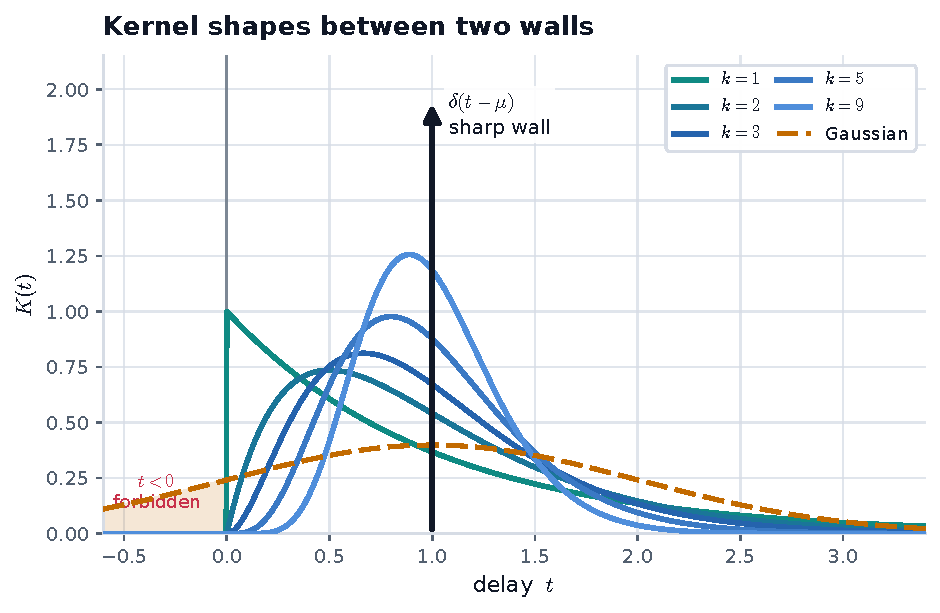
\includegraphics[width=\linewidth]{fig1_kernel_gallery.pdf}
\caption{Passive causal kernel shapes. Gamma kernels of fixed mean $\mu=1$ and increasing shape $k$ interpolate from skewed toward bell-shaped while staying supported on $[0,\infty)$. The delta $\delta(t-\mu)$ marks the sharp wall ($N=0$); the variance-matched Gaussian for the broadest case (dashed) marks the efficient wall ($N=\sigma^2$), unreachable as its mass leaks to $t<0$ (shaded). Shown as a one-parameter slice through the kernel space, not a literal path between the walls.}
\label{fig:kernel-gallery}
\end{figure}

The composition law for $N$ is not an equality.

\begin{theorem}[Strict entropy-power spreading]\label{thm:epi}
Let $K_1,K_2$ be passive causal temporal kernels with finite differential entropy, each carrying a density rather than a point mass. Then
\begin{equation}\label{eq:epi}
N(K_2*K_1)\ \ge\ N(K_1)+N(K_2),
\end{equation}
and the inequality is strict,
\[
N(K_2*K_1)\ >\ N(K_1)+N(K_2).
\]
\end{theorem}

\begin{proof}
By Proposition~\ref{thm:spread}, each $K_i$ is the law of an independent nonnegative delay $T_i$, and $K_2*K_1$ is the law of $T_1+T_2$. Inequality \eqref{eq:epi} is the Shannon--Stam entropy power inequality \cite{stam1959,blachman1965}. Equality there holds if and only if $T_1$ and $T_2$ are Gaussian. But a random variable whose density is supported on $[0,\infty)$ cannot be Gaussian, since the Gaussian law charges the whole real line. Equality is therefore unattainable for passive causal kernels, and the inequality is strict. The same support argument applied to \eqref{eq:Npbound} makes that bound strict as well.
\end{proof}

The contrast with Proposition~\ref{thm:spread} is the whole point. Variance adds exactly, so the second-moment statement of irreversibility is neutral: it forbids sharpening but is indifferent to the act of composing. Entropy power instead \emph{strictly increases beyond additivity} at every nontrivial stage. Cascaded causal mediation does not merely fail to sharpen the response; it produces strictly more dispersion than the sum of its parts, and it does so precisely because causality forbids the one shape---the Gaussian---for which composition would be efficient.

This sharpens the boundary picture into two boundaries. The interior of the passive causal kernel space is pinned below by the delta locus $N=0$ (infinitely sharp, reached only in the limit) and, through \eqref{eq:Npbound}, above by the Gaussian locus $N=\sigma^2$ (maximally efficient spread, where the entropy power inequality would close). Causal kernels live strictly between the two: never perfectly sharp, never perfectly efficient. Both ideals sit on the boundary, and the physics happens in between.

The strict gap is order-unity, not marginal: a single exponential stage has $N/\sigma^2=e/(2\pi)\approx0.43$, so the first composition already adds about $57\%$ of a stage's variance beyond additivity (Fig.~\ref{fig:entropy-power-plane}).

\begin{figure}[t]
\centering
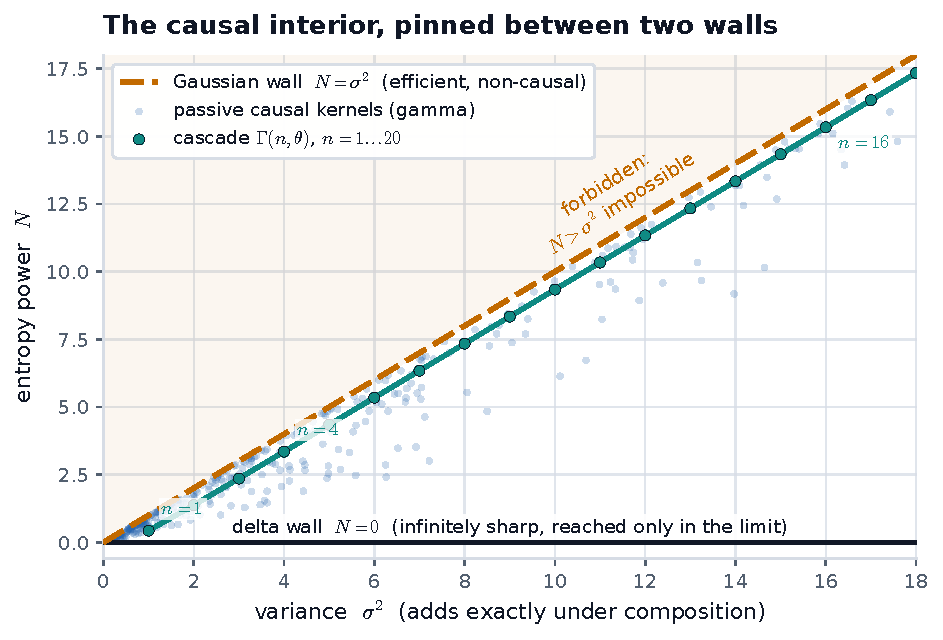
\includegraphics[width=\linewidth]{fig4_entropy_power_plane.pdf}
\caption{The causal interior between two walls. Entropy power $N$ vs variance $\sigma^2$. The Gaussian locus $N=\sigma^2$ (dashed) and delta locus $N=0$ bound the admissible region; causal gamma kernels fill the strict interior. The cascade $\Gamma(n,\theta)$ climbs toward the Gaussian wall, reaching $N/\sigma^2\approx0.96$ at $n=16$ without equality.}
\label{fig:entropy-power-plane}
\end{figure}

The diffusive kernel of \S2 is the flow that carries a response into that interior. Writing the profile of \eqref{eq:diffusive} as $p(\cdot,\tau)$, it solves the heat equation $\partial_\tau p=D\,\Delta p$, and de Bruijn's identity gives the entropy production rate exactly \cite{dembo1991}:
\begin{equation}\label{eq:debruijn}
\frac{d}{d\tau}\,h\bigl(p(\cdot,\tau)\bigr)=D\,J\bigl(p(\cdot,\tau)\bigr),
\qquad
J(p)=\int \frac{\|\nabla p\|^2}{p}\,d\xi,
\end{equation}
with $J$ the Fisher information of the current profile. Since $J\ge0$, diffusion increases entropy monotonically, at a rate set by $J$. The discrete statement---each passive stage strictly adds entropy power---and the continuous one---diffusion is the generator of entropy increase---are the same irreversibility read at two resolutions.

\section{Finite-speed corollary and interpretation}

For space-time kernels, let the causal cone condition be
\begin{equation}\label{eq:cone}
G(\xi,\tau)=0
\quad\text{unless}\quad
\tau\ge0,
\qquad \|\xi\|\le c\tau.
\end{equation}

\begin{corollary}[Cone closure]
If $G_1$ and $G_2$ satisfy \eqref{eq:cone}, then every convex mixture
$(1-\lambda)G_1+\lambda G_2$ also satisfies \eqref{eq:cone}. Moreover,
their convolution satisfies \eqref{eq:cone}.
\end{corollary}

\begin{proof}
The mixture statement is immediate from support inclusion. For convolution, any nonzero contribution factors through increments $(\xi_1,\tau_1)$ and $(\xi_2,\tau_2)$ with $\xi=\xi_1+\xi_2$ and $\tau=\tau_1+\tau_2$. Since $\|\xi_i\|\le c\tau_i$,
\[
\|\xi\|\le \|\xi_1\|+\|\xi_2\|
\le c(\tau_1+\tau_2)=c\tau.
\]
Thus the composed kernel remains inside the cone.
\end{proof}

\section{Conclusion}

The resulting picture is a small geometry of mediation kernels. The instantaneous local kernel $\delta(\xi)\delta(\tau)$ is a singular idealization. Ballistic kernels concentrate response on causal arrival surfaces. Diffusive kernels distribute response across many small randomized delays. Lossy kernels reduce total gain; active kernels require an external energy source. But passive causal kernels have stable algebraic structure: they may be mixed, composed, and decomposed into channels and stages without violating causality.

A jump in acceleration is therefore the boundary case obtained when the mediating kernel collapses to a delta. Real finite-response dynamics correspond to interior points of a constrained kernel space. The proposition gives one precise sense in which moving into that interior is irreversible under passive composition: additional hidden mediation stages add spread rather than remove it. The entropy-power refinement makes the irreversibility strict and gives it a second wall to face: the response can approach neither the infinitely sharp delta nor the maximally efficient Gaussian, and diffusion is exactly the flow that drives entropy upward between them. Sharpness is not destroyed; it is revealed as an ideal boundary of causal response.

{\small
\setlength{\parskip}{0.12em}
\begin{thebibliography}{9}
\setlength{\itemsep}{0.08em}

\bibitem{applebaum2009}
D. Applebaum, \emph{Levy Processes and Stochastic Calculus}, 2nd ed.,
Cambridge University Press, 2009.

\bibitem{barron1986}
A. R. Barron, ``Entropy and the central limit theorem,''
\emph{Annals of Probability} \textbf{14}(1), 336--342, 1986.

\bibitem{blachman1965}
N. M. Blachman, ``The convolution inequality for entropy powers,''
\emph{IEEE Transactions on Information Theory} \textbf{11}(2), 267--271, 1965.

\bibitem{dembo1991}
A. Dembo, T. M. Cover, and J. A. Thomas, ``Information theoretic inequalities,''
\emph{IEEE Transactions on Information Theory} \textbf{37}(6), 1501--1518, 1991.

\bibitem{shannon1948}
C. E. Shannon, ``A mathematical theory of communication,''
\emph{Bell System Technical Journal} \textbf{27}, 379--423 and 623--656, 1948.

\bibitem{stam1959}
A. J. Stam, ``Some inequalities satisfied by the quantities of information of
Fisher and Shannon,'' \emph{Information and Control} \textbf{2}(2), 101--112, 1959.

\end{thebibliography}
}

\end{document}
